
\section{Introduction à l’informatique}
\subsection{Objectifs généraux}

L'objectif de ce module est, avant tout, d'apporter des compétences de réflexion pour la résolution de problèmes. En effet, écrire un code informatique, c'est d'abord écrire un algorithme qui répond à une problématique.

Durant ce module, nous verrons le langage C car il est suffisamment bas niveau pour illustrer le fonctionnement des systèmes informatiques. C'est, par ailleurs, le langage utilisé pour développer les systèmes embarqués.


\subsection{Systèmes de comptage}
\subsubsection{Le système unaire}

Quand on compte sur nos doigts, on utilise un système \textbf{unaire} (base 1) :
\begin{itemize}
	\item Chaque doigt levé représente une unité.
	\item Exemple : 3 doigts levés = le nombre 3.
\end{itemize}

\subsubsection{Le système binaire}

En binaire, chaque chiffre (appelé \textbf{bit}) peut prendre deux valeurs :
\begin{itemize}
	\item \texttt{0} → inactif, éteint, faux
	\item \texttt{1} → actif, allumé, vrai
\end{itemize}

\begin{UPSTIinfor}{Exemple des ampoules}
	Si on a \textbf{3 ampoules} qui peuvent être allumées (1) ou éteintes (0) :
	\begin{itemize}
		\item \texttt{000} = 0
		\item \texttt{001} = 1
		\item \texttt{010} = 2
		\item ...
		\item \texttt{111} = 7
	\end{itemize}

	Avec 3 ampoules, on peut donc compter de 0 à 7.
\end{UPSTIinfor}

\begin{UPSTIinfor}{A retenir : Le binaire en informatique}
	Tous les systèmes informatiques utilisent le binare pour encoder toutes les informations
	Les données sont stoquée grâce à des \textbf{transistors} qui se comportent comme de minuscules interrupteurs.
\end{UPSTIinfor}

\subsubsection{L’octet}

Historiquement, les données étaient envoyées par groupes de 8 bits sur les bus des premiers processeurs.
Ces groupes ont été appelés des \texttt{octet} (\texttt{oct} pour "huit" et \texttt{et} pour "petit").
C'est depuis devenu une unité de mesure de la taille des données (octet, kilo-octet, Mega-octet, etc.).

\begin{UPSTIinfor}{A retenir : Un octet (byte)}
	Un octet est un groupe de huit bits. Il peut représenter 256 valeurs différentes (de 0 à 255).
	\begin{itemize}
		\item Exemple :
		      \begin{itemize}
			      \item \texttt{00000101} = 5
			      \item \texttt{11111111} = 255
		      \end{itemize}
	\end{itemize}
\end{UPSTIinfor}

\subsubsection{Conversion en décimal}
Chaque bit a un \textbf{poids} qui correspond à une puissance de 2 :

\begin{center}
	\begin{tabular}{|l|l|l|l|l|l|l|l|}
		\hline
		\makecell[tl]{$2^{7}$         \\ 128} & \makecell[tl]{$2^{6}$\\  32} & \makecell[tl]{$2^{5}$\\ 64} & \makecell[tl]{$2^{4}$\\ 16} & \makecell[tl]{$2^{3}$\\ 8} & \makecell[tl]{$2^{2}$ \\ 4} & \makecell[tl]{$2^{1}$\\ 2} & \makecell[tl]{$2^{0}$ \\1} \\
		\hline
		0 & 0 & 0 & 0 & 0 & 0 & 0 & 0 \\
		\hline
	\end{tabular}
\end{center}
\begin{UPSTIinfor}{Exemple}
	\begin{center}
		\begin{tabular}{|l|l|l|l|l|l|l|l|}
			\hline
			\makecell[tl]{$2^{7}$         \\ 128} & \makecell[tl]{$2^{6}$\\  32} & \makecell[tl]{$2^{5}$\\ 64} & \makecell[tl]{$2^{4}$\\ 16} & \makecell[tl]{$2^{3}$\\ 8} & \makecell[tl]{$2^{2}$ \\ 4} & \makecell[tl]{$2^{1}$\\ 2} & \makecell[tl]{$2^{0}$ \\1} \\
			\hline
			0 & 1 & 0 & 0 & 1 & 0 & 0 & 1 \\
			\hline
		\end{tabular}
	\end{center}
	\texttt{01001001} = 64 + 8 + 1 = \textbf{73}
\end{UPSTIinfor}

\subsection{Représentation de l’information}
Pour résumer : un système informatique n'a qu'une seule façon d'encoder une information : le binaire.

Pour chaque type de données, une convention est mise en place pour savoir comment un ordinateur comprendra cette information.
Que ce soit pour manipuler un nombre entier, un nombre à virgule, du texte, une image, une vidéo, du sons, ou n'importe quel type de donnée, un système informatique utilisera des 0 et des 1 pour le représenter.

Quelques exemples sont donnés dans cette section
\subsubsection{ASCII : Représenter du texte}

\begin{itemize}
	\item Les lettres peuvent être codées en binaire via la norme \textbf{ASCII}, qui associe des nombres aux caractères. Par exemple, \texttt{A} correspond à 65 : \texttt{01000001}.
	\item Exemple : un message texte pourrait avoir pour valeurs binaires 72, 73 et 33, correspondant aux caractères \texttt{H}, \texttt{I} et \texttt{!}.
	\item La Figure~\ref{table-ascii} représente cette table ASCII.
\end{itemize}

\begin{figure}[h!t]
	\centering
	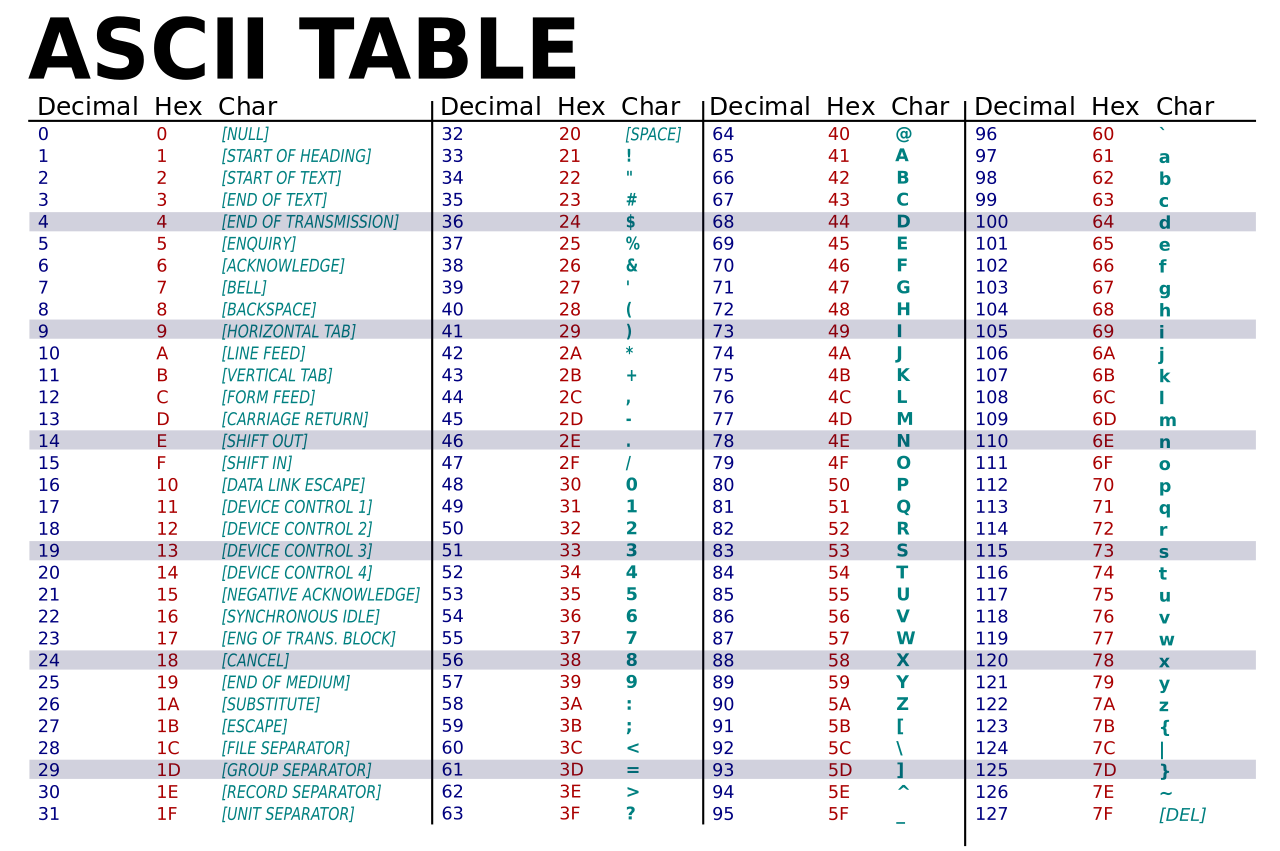
\includegraphics[width=0.8\textwidth]{ASCII-Table.png}
	\caption{Table ASCII}
	\label{table-ascii}
\end{figure}

\subsubsection{Unicode : Représenter plus de caractères}

\begin{itemize}
	\item Le binaire traditionnel ne permettait pas de représenter tous les caractères humains. \textbf{Unicode} a donc étendu ce système (plus de bits), intégrant notamment les lettre avec accents, les symbôles de nombreuse langues ainsi que des emoji.
	\item Chaque plate-forme peut afficher les emoji différemment.
\end{itemize}

\subsubsection{RGB : Représenter les couleurs}

\begin{itemize}
	\item Les images numériques se construisent à partir de trois composantes : Rouge, Vert, Bleu (\textbf{RGB}).
	\item Si on prend les valeurs 72, 73 et 33 (les mêmes que pour “HI!”), on obtient une nuance de jaune clair.
	\item Une image est simplement une collection de ces valeurs RGB. Une vidéo = une séquence d’images. La musique peut être codée de manière similaire.
\end{itemize}


\subsection{Les algorithmes}

Un \textbf{algorithme} est une suite d’instructions permettant de résoudre un problème.

\begin{UPSTIinfor}{Propriétés d’un algorithme}
	\begin{itemize}
		\item Il doit être \textbf{fini} (il s’arrête).
		\item Il doit être \textbf{précis} (chaque étape est claire).
		\item Il doit être \textbf{réalisable} par une machine.
	\end{itemize}
\end{UPSTIinfor}

\subsubsection{Exemples d’algorithmes}

\begin{itemize}
	\item \textbf{Dans la vie quotidienne :}
	      \begin{itemize}
		      \item Une recette de cuisine (étapes précises à suivre).
		      \item Changer une roue (suite d’actions logiques).
	      \end{itemize}
\end{itemize}

\begin{itemize}
	\item \textbf{En informatique :}
	      \begin{itemize}
		      \item Trier des cartes par ordre croissant.
		      \item Chercher un nom dans un annuaire.
	      \end{itemize}
\end{itemize}

\begin{UPSTIinfor}{Algorithme de recherche dichotomique}
	\begin{enumerate}
		\item Ouvrir l’annuaire au milieu.
		\item Si le nom cherché est avant, prendre la moitié gauche.
		\item Sinon, prendre la moitié droite.
		\item Répéter jusqu’à trouver le nom.
	\end{enumerate}
\end{UPSTIinfor}

C’est un \textbf{algorithme efficace} : au lieu de parcourir chaque nom un par un, on élimine la moitié des candidats à chaque étape.